%!TEX root = ../thesis.tex
%*******************************************************************************
%*********************************** Analysis Overview *********
%*******************************************************************************

\chapter{Analysis overview}\label{ch:1lepton}

\ifpdf
    \graphicspath{{chapter-analysis/Figs/Raster/}{chapter-analysis/Figs/PDF/}{chapter-analysis/Figs/}}
\else
    \graphicspath{{chapter-analysis/Figs/Vector/}{chapter-analysis/Figs/}}
\fi


This chapter aims to give an introduction to the search for electroweakinos presented in this work. First, the targeted final state, the 1-lepton final state, is introduced and motivated, followed by the \gls{sm} background processes that need to be considered when doing searches for \gls{susy} in this final state. Next the reconstruction and identification of physics objects as well as the event selection requirements are described.

\section{Search for electroweakinos in the 1-lepton final state}

In the search for electroweakinos presented herein, the simplified model introduced in \cref{sec:models_used} is interpreted in final states with one lepton, two \textit{b}-jets and high missing transverse momentum. This final state can occur when the $W$ boson decays through $W^\pm\rightarrow\ell^\pm\nu_\ell$, while the Higgs boson decays into $h\rightarrow b\bar{b}$. Although a final state without leptons would benefit from the higher branching fraction of the $W^\pm\rightarrow q'\bar{q}$ decay, due to the \gls{qcd} couplings these final states are largely dominated by \gls{qcd} multi-jet background processes that are omnipresent at hadron colliders like the \gls{lhc}. Final states with exactly one lepton have lower cross sections but allow to reject a majority of the \gls{qcd} background, as pure \gls{qcd} multi-jet events can only appear in the 1-lepton final state through false reconstruction of a jet as a lepton (so-called \textit{fake} leptons). 

Targeting the decay of the Higgs boson into a pair of \textit{b} quarks benefits from the high branching ratio of 58.3\% and allows a full reconstruction of Higgs candidates, a procedure that will be used to achieve a high signal-to-background ratio. \improvement{refer to observables}. \Cref{fig:Wh_model_full} shows the full signal model targeted in this search, including the considered decays of the $W$ and Higgs bosons. 

Previous searches for electroweakinos in this final state have been performed by the ATLAS~\cite{SUSY-2013-23,SUSY-2017-01} and CMS~\cite{CMS-SUS-16-043} collaborations, excluding $\charg\neutr$ masses up to $\SI{540}{\GeV}$ and $\SI{490}{\GeV}$, respectively, for massless $\lsp$. The two previous ATLAS searches used $\SI{20.3}{\per\femto\barn}$ of $\sqrt{s}=\SI{8}{\TeV}$ and $\SI{36.1}{\per\femto\barn}$ of $\sqrt{s}=\SI{13}{\TeV}$ $pp$ collision data, respectively. As opposed to this, the search presented in the following uses the full dataset available from the Run~2 data taking period, amounting to an unprecedented $\SI{139}{\per\femto\barn}$ of $pp$ collision data at $\sqrt{s}=\SI{13}{\TeV}$.

\begin{figure}
	\centering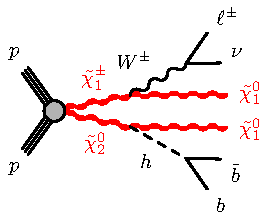
\includegraphics[width=.4\textwidth]{model_c1n2_Wh}
	\caption{Diagram for the simplified model used in this work including the decays $W^\pm\rightarrow\ell^\pm\nu_\ell$ and $h\rightarrow b\bar{b}$.}\label{fig:Wh_model_full}
\end{figure}

\section{Standard Model backgrounds}

Although the requirement of exactly one lepton isolated from surrounding hadronic activity significantly reduces the contribution from \gls{qcd} multi-jet background, numerous \gls{sm} processes can result in final states with exactly one isolated lepton, multiple jets and missing transverse momentum. Background sources are generally classified into \textit{reducible} and \textit{irreducible} backgrounds. Irreducible backgrounds are processes that have a physical phase space that is indistinguishable from the final state of the signal process considered. Reducible backgrounds, on the other hand, result from partially misreconstructed processes as well as mismeasurements. Examples of reducible processes are events where a lepton originates from a \gls{hf} decay, photon conversions or misreconstructed jets. \gls{sm} processes that result in final states with an isolated lepton, multiple jets and missing transverse momentum typically involve a $W$ boson decaying into a lepton--neutrino pair (a so-called \textit{leptonic decay}). The neutrino will contribute to the total missing transverse momentum in the event, while additional jets can appear in the final state through \gls{qcd} radiation or other branches of the decay chain.

By far the largest \gls{sm} background contributions stem from the production of top quarks, predominantly through top quark pair $\ttbar$ production, where both top quarks decay into a $W$ boson and a $b$ quark. Final states with one isolated lepton can occur through leptonic decay of one of the $W$ bosons. \Cref{fig:ttbar} shows a diagram depicting an exemplary decay of a $\ttbar$ system into a final state with one lepton, multiple jets (two of which originate from \textit{b} quarks) and missing transverse momentum. In addition to $\ttbar$, single top production (\textit{s}-channel, \texttt{t}-channel or \textit{tW}-channel) can also result in similar final states as the \gls{susy} signal and thus constitutes a significant \gls{sm} background process. An exemplary decay is shown in~\cref{fig:singletop}.

Apart from processes involving top quarks, the production of a $W$ boson in association with multiple jets ($\wjets$) is the third major background considered in the analysis. If the $W$ boson undergoes a leptonic decay and two of the produced jets are tagged as originating from $b$ quarks, the signature of this process is similar to that of signal events. An exemplary diagram for a $\wjets$ event is shown in~\cref{fig:wjets}. 

Production of multiple vector bosons $V$ ($=W,Z$)---although not a dominant background due to low cross sections---can still result in the same final state as the signal process. In the following, diboson $VV$ and multibosons $VVV$ processes are considered.

Other \gls{sm} backgrounds with small contributions in the phases spaces targeted by the analysis include $Z+\mathrm{jets}$ production, $\ttbar+V$ production, as well as various processes involving Higgs bosons. $Z+\mathrm{jets}$ plays only a minor role, as the only irreducible component is $Z(\rightarrow\tau\tau)+\mathrm{jets}$, where one $\tau$-lepton undergoes a leptonic decay and the other one a hadronic decay. Production of $\ttbar+V$ has a similar topology as ordinary $\ttbar$ processes but with lower cross section and additional objects in the final state. Higgs processes considered in the following include single Higgs production through \gls{vbf} or \gls{ggf} as well as $h+V$ and $h+\ttbar$ processes. In the following, these backgrounds are simply labelled \textit{other}. 

Pure \gls{qcd} multi-jet events can only appear in the 1-lepton final state through false reconstruction of a jet as a lepton (so-called \textit{fake} leptons) and mismeasurement of $\etmiss$. As it has been shown that this background is negligible in all selections relevant to this search, no estimation for \gls{qcd} contribution is considered in the following~\cite{SUSY-2019-08}.

\begin{figure}
	\centering
	\begin{subfigure}[b]{0.3\linewidth}
		\centering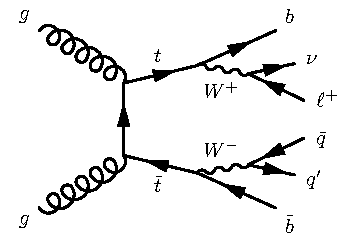
\includegraphics[width=\textwidth]{ttbar}
		\caption{\label{fig:ttbar}}
	\end{subfigure}\quad
		\begin{subfigure}[b]{0.3\linewidth}
		\centering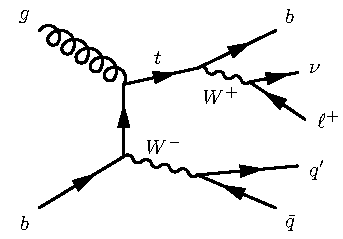
\includegraphics[width=\textwidth]{singletop}
		\caption{\label{fig:singletop}}
	\end{subfigure}\quad
	\begin{subfigure}[b]{0.3\linewidth}
		\centering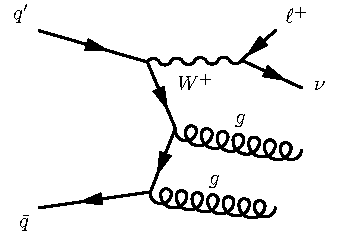
\includegraphics[width=\textwidth]{wjets}
		\caption{\label{fig:wjets}}
	\end{subfigure}
%	\begin{subfigure}[b]{0.25\linewidth}
%		\centering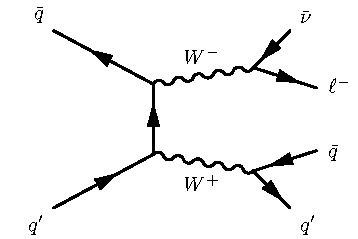
\includegraphics[width=\textwidth]{diboson}
%		\caption{\label{fig:diboson}}
%	\end{subfigure}
	\caption{Exemplary Feynman diagrams showing the dominant processes \subref{fig:ttbar} $t\bar{t}$, \subref{fig:singletop} single top and \subref{fig:wjets} $W+\textrm{jets}$ production with subsequent decays.}
	\label{fig:sm_backgrounds_feynman}
\end{figure}


\section{Monte Carlo samples}

\Cref{tab:mc_generators} summarises all \gls{mc} generators and software versions used for the simulated events used in the following. Further details are given in the relevant ATLAS simulation notes~\cite{ATL-PHYS-PUB-2018-009,ATL-PHYS-PUB-2016-005,ATL-PHYS-PUB-2017-006,ATL-PHYS-PUB-2017-005,ATL-PHYS-PUB-2016-002}.

\subsection{Signal samples}

The $\charg\neutr$ pair production signal samples were generated at \gls{lo} using \textsc{MadGraph5\_aMC@NLO} 2.6.2~\cite{MGaMCNLO:2014hca,Frederix:2012ps} with up to two additional partons in the \gls{me}. \textsc{MadGraph5\_aMC@NLO} is interfaced with \textsc{Pythia8}~\cite{Pythia8:2007gs} for the \gls{ps}, hadronisation and underlying event, using the CKKW-L~\cite{Lonnblad:2011xx} scheme for matching the \gls{ps} to the \glspl{me}. The NNPDF 2.3 LO~\cite{Ball:2012cx} \gls{PDF} set and the A14 set of tuned parameters~\cite{ATL-PHYS-PUB-2014-021} are used. For modelling the decay of \gls{hf} quarks, \textsc{EvtGen}~\cite{Lange:2001uf} v1.6 is used. 

As the $\charg/\neutr$ and $\lsp$ masses are free parameters of the signal model, they are systematically scanned, resulting in a set of 164 distinct evenly distributed in the two-dimensional grid spanned by the mass parameters. In the following the two-dimensional grid will be referred to as \textit{signal grid}, while the distinct signal scenarios (each witch a unique set of mass parameter values) will be referred to as \textit{signal point}. The generated signal grid covers $\charg/\neutr$ masses from $\SI{150}{\GeV}$ to $\SI{1.1}{\TeV}$ and $\lsp$ masses from $\SI{0}{\GeV}$ to $\SI{550}{\GeV}$, avoiding the kinematically forbidden region with $m(\charg/\neutr) > m(\lsp) + m(h)$.

Signal samples well within the expected sensitivity range of the analysis (with relatively low $\charg/\neutr$ and $\lsp$ masses) are generated using the \textsc{ATLFAST-II} detector simulation, while the full detector simulation using \textsc{Geant4} is used for the remaining model points for maximum accuracy. In order to account for pileup effects, all signal samples are overlaid with simulated minimum bias events generated using \textsc{Pythia8} and the A3 tune~\cite{ATL-PHYS-PUB-2016-017}, reweighted to match the pileup distribution measured in data. 

The cross sections for chargino pair production have been calculated using \textsc{Resummino}~\cite{Fuks:2013vua} at \gls{nlo} in the strong coupling constant and including \gls{nll} terms in the soft gluon resummation~\cite{Fiaschi:2018hgm,Fuks:2012qx}.

\subsection{Background samples}

Top pair production and single top processes were generated using \textsc{Powheg-Box} v2~\cite{PowhegBox:2010xd}, implementing the \textsc{POWHEG} method~\cite{Powheg1,Powheg2} for merging \gls{nlo} \glspl{me} with the \glspl{ps}. The \gls{ps}, hadronisation and underlying event were simulated using \textsc{Pythia8} with the A14 tune. Production of $\ttbar$ in association with a vector boson $\ttbar+V$ are generated using \textsc{MadGraph5\_aMC@NLO} 2.3.3, interfaced with \textsc{Pythia8} for the \gls{ps}. The set of \glspl{PDF} used for simulation of $\ttbar$, single top, and $\ttbar+V$ is the NNPDF2.3LO set.

Production of a vector boson $V$ with additional jets ($V+\mathrm{jets}$) is simulated using \textsc{Sherpa} 2.2.1~\cite{Gleisberg:2008ta,Bothmann:2019yzt}, allowing up to two (four) additional parton emissions at NLO (LO) accuracy. The CKKW \gls{me}+\gls{ps} matching and merging scheme~\cite{Hoeche:2009rj,Catani:2001cc}, extended to NLO accuracy~\cite{Hoeche:2012yf}. Diboson ($VV$) and multiboson ($VV$) is simulated using \textsc{Sherpa} 2.2.1 and 2.2.2. The \glspl{PDF} used are provided by the NNPDF3.0NNLO set~\cite{Ball:2014uwa} and the generator tune is the default \textsc{Sherpa} tune.

All Higgs processes are simulated using \textsc{Powheg-Box} v2 for the \gls{me} calculations and \textsc{Pythia8} for the \gls{ps}, underlying event and hadronisation. While the generation of $h+\ttbar$ uses the A14 tune and the NNPDF2.3LO set, $h+V$ and single Higgs production are simulated using the NNPDF 3.0 NNLO set and the AZNLO~\cite{ATL-PHYS-PUB-2013-017} set of tuned generator parameters.

The detector simulation for all \gls{mc} background samples was performed using the full detector simulation based on \textsc{Geant4}, introduced in \cref{sec:detector_simulation}. Except for the \gls{mc} samples generated using \textsc{Sherpa}, all background samples use \textsc{EvtGen} v1.2 or v1.6 to model the decay of \gls{hf} quarks. Similar to the signal models, all background samples are mixed with simulated minimum bias events generated with \textsc{Pythia8} and the A3 tune.

\begin{table}
	\centering
	\setlength\heavyrulewidth{0.2ex}
	\small
	\caption{Overview of configuration of \gls{mc} generators used for simulating the various signal and \gls{sm} background processes.}
	\resizebox{\textwidth}{!}{\begin{tabular} {llllll}
	\toprule
	Process & Matrix element & Parton shower & PDF set & Cross section & Tune\\ 
	\midrule
	Signal & \textsc{MadGraph5\_aMC@NLO} 2.6.2 & \textsc{Pythia} 8.230 & NNPDF 2.3 LO & NLO+NLL~\cite{Fuks:2013vua,Fiaschi:2018hgm,Fuks:2012qx} & A14 \\
	\midrule	
	$\ttbar$ & \textsc{Powheg-Box} & \textsc{Pythia} 8.230 & NNPDF2.3LO & NNLO+NNLL~\cite{Czakon:2011xx,Cacciari:2011hy} & A14 \\
	$t$ (s-channel) & \textsc{Powheg-Box} & \textsc{Pythia} 8.230 & NNPDF2.3LO & NLO~\cite{Kant:2014oha} & A14 \\
	$t$ (t-channel) & \textsc{Powheg-Box} & \textsc{Pythia} 8.230 & NNPDF2.3LO & NLO~\cite{Kant:2014oha} & A14 \\
	$t+W$ & \textsc{Powheg-Box} & \textsc{Pythia} 8.230 & NNPDF2.3LO & NNLO~\cite{Kant:2014oha,Kidonakis:2010ux,} & A14 \\
	$\ttbar + V$ & \textsc{MadGraph5\_aMC@NLO} 2.3.3 & \textsc{Pythia} 8.210 & NNPDF2.3LO & NLO~\cite{Campbell:2012dh,Lazopoulos:2008de} & A14 \\
	\midrule
	$V+\mathrm{jets}$ & \multicolumn{2}{c}{\textsc{Sherpa} 2.2.1} & NNPDF3.0NNLO & NNLO~\cite{Gavin:2010az} & \textsc{Sherpa} default \\
	$VV$ & \multicolumn{2}{c}{\textsc{Sherpa} 2.2.1/2.2.2} & NNPDF3.0NNLO & NLO~\cite{ATL-PHYS-PUB-2017-005} & \textsc{Sherpa} default\\
	$VVV$ & \multicolumn{2}{c}{\textsc{Sherpa} 2.2.1/2.2.2} & NNPDF3.0NNLO & NLO~\cite{ATL-PHYS-PUB-2017-005} & \textsc{Sherpa} default\\
	\midrule
	$h+\ttbar$ & \textsc{Powheg-Box} & \textsc{Pythia} 8.230 & NNPDF2.3LO & NLO~\cite{deFlorian:2016spz} & A14 \\
	$h+V$ & \textsc{Powheg-Box} & \textsc{Pythia} 8.212 & NNPDF3.0NNLO & NNLO~\cite{deFlorian:2016spz} & AZNLO \\
	\textit{h (ggF)} & \textsc{Powheg-Box} & \textsc{Pythia} 8.212 & NNPDF3.0NNLO & N$^3$LO+N$^3$LL~\cite{deFlorian:2016spz} & AZNLO \\
	\textit{h (VBF)} & \textsc{Powheg-Box} & \textsc{Pythia} 8.212 & NNPDF3.0NNLO & NNLO~\cite{deFlorian:2016spz} & AZNLO \\
	\bottomrule
	\end{tabular}}\vspace{3mm}
	\label{tab:mc_generators}   
\end{table}

\section{Object definitions}

\subsection{Electrons}

\subsection{Muons}

\subsection{Jets}

\subsection{\textit{b}-tagging}

\section{Overlap removal}

\section{Event selection}

\section{Triggers}